%--------------PREAMBLE----------------------------------------------------------------------


\documentclass[12pt]{beamer}
\usetheme{boadilla}


\usepackage{ulem,bm,amsmath,bbm,amsfonts,nicefrac,latexsym,amsmath,amsfonts,amsbsy,amscd,amsxtra,amsgen,amsopn,bbm,amsthm,amssymb,graphicx} % you may include additional packages should you need them




\newcommand{\R}{\mathbb{R}}    % the real numbers


\title{Understanding the Information Content in Diverse Observations of Forest Carbon Stocks and Fluxes for Data Assimilation and Ecological Modeling\\ NERC case partnership with Forest Research}
\author{Ewan Pinnington}


\begin{document}



%--------------TITLE SLIDE-----------------------------------------------------------------
\frame{

\maketitle

}

%--------------Contents SLIDE-----------------------------------------------------------------
%\frame{
 %\frametitle{Outline}
  %\small
  %\tableofcontents[hideothersubsections]
  %\normalsize
%\tableofcontents
%\makeindex
%}

%--------------SLIDE 1-----------------------------------------------------------------
\section{The DALEC model}
\frame{\frametitle{The DALEC Model}

The DALEC model is a simple process-based model describing the carbon balance of an evergreen forest ecosystem . The model is constructed of five carbon pools linked via fluxes. 

\pause

\begin{figure}[h!]
    \centering
    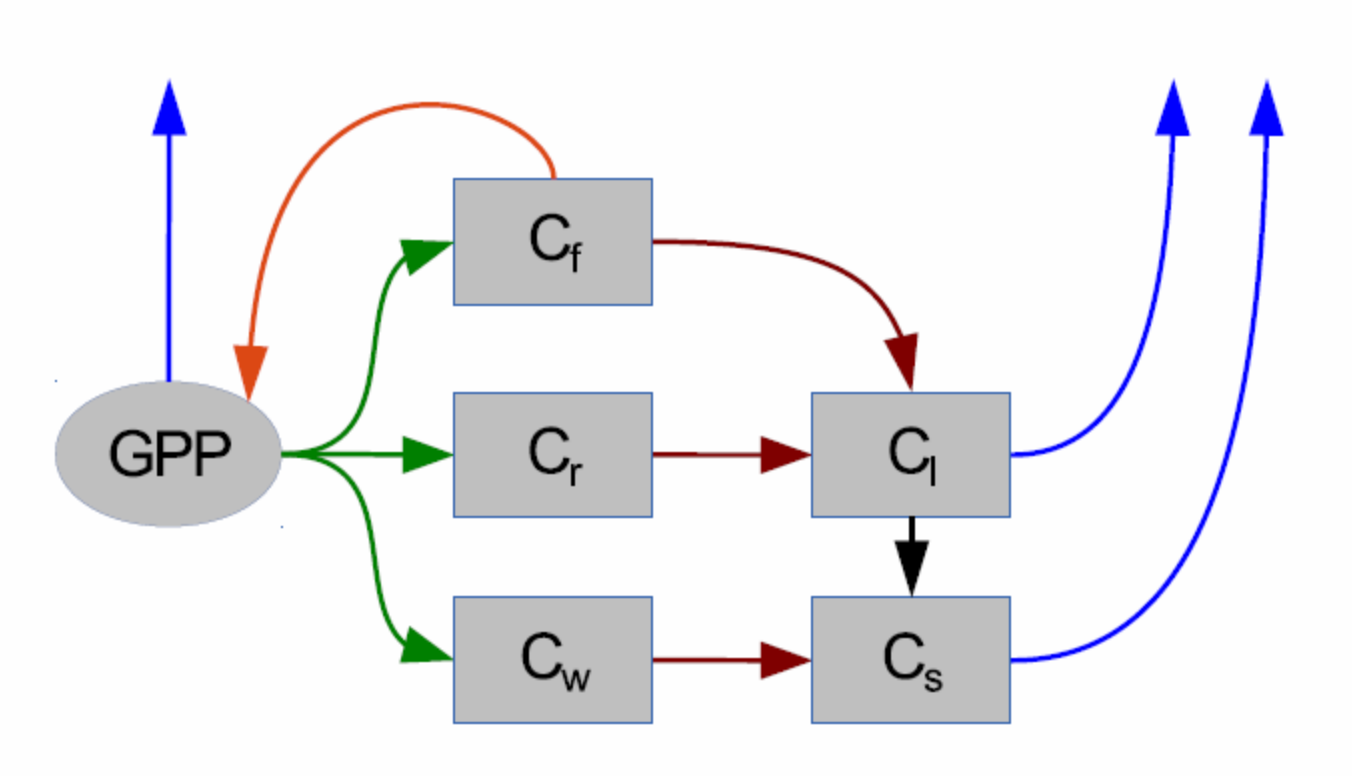
\includegraphics[width=0.5\textwidth]{DALECpic.png}
    \caption{DALEC carbon balance model, (foliage ($C_f$), fine roots ($C_r$), woody biomass ($C_w$), litter ($C_l$) and soil organic matter ($C_s$)). The gross primary production function ($GPP$) uses meteorological driving data and the site's leaf area index (a function of $C_f$) to calculate the total amount of carbon to be allocated at a daily time step. }
    \label{fig:DALEC_mod}
\end{figure}

}


%--------------SLIDE 3-----------------------------------------------------------------
\section{Deriving the Hermite Polynomials} 
\frame{\frametitle{DALEC model equations}
The model equations for the carbon pools at day $t+1$ are as follows:

\begin{align}
\small C_f(t+1)&=(1-p_5)C_f(t)+p_3(1-p_2)GPP(C_f(t),\phi),
 \\C_r(t+1)&=(1-p_7)C_r(t)+p_4(1-p_3)(1-p_2)GPP(C_f(t),\phi), 
\\C_w(t+1)&=(1-p_6)C_w(t)+(1-p_4)(1-p_3)(1-p_2)GPP(C_f(t),\phi), 
 \\C_l(t+1)&=(1-(p_1+p_8)T(t))C_l(t)+p_5C_f(t)+p_7C_r(t), 
 \\C_s(t+1)&=(1-p_9T(t))C_s+p_6C_w(t)+p_1T(t)C_l(t),
\end{align}

where $T(t)=\frac{1}{2}exp(p_{10}T_m(t))$, $T_m$ is daily mean temperature, $p_1,\ldots,p_{10}$ are rate parameters and $\phi$ represents the meteorological driving data used in the $GPP$ function.
}


%--------------SLIDE 4-----------------------------------------------------------------

\frame{\frametitle{DALEC Tangent Linear Model}
To compute the tangent linear model for DALEC ($\textbf{M}_i=\frac{\delta \underline{m}_i}{\delta \underline{x}_i}$) using a state vector, $\underline{x} = (C_f, C_r, C_w, C_l, C_s)$, we first need to compute the first derivative of  $GPP$.
 
}

%--------------SLIDE 5-----------------------------------------------------------------

\frame{
We then have,
\begin{align*} 
&\textbf{M}_i =
\\& \scriptsize\begin{pmatrix} 
(1-p_5)+p_3(1-p_2)\zeta & 0 & 0 & 0 & 0 \\
p_4(1-p_3)(1-p_2)\zeta & (1-p_7) & 0 & 0 & 0 \\
(1-p_4)(1-p_3)(1-p_2)\zeta & 0 & (1-p_6) & 0 & 0 \\
p_5 & p_7 & 0 & (1-(p_1+p_8)T(t)) & 0 \\
0 & 0 & p_6 & p_1T(t) & (1-p_9T(t)) \\
\end{pmatrix},
\end{align*}

where $\zeta=GPP'(C_f(t),\phi)$.
}

%--------------SLIDE 6-----------------------------------------------------------------

\frame{\frametitle{4DVAR with DALEC}
We can now code up a 4DVAR cost function and gradient where,

\begin{align*}
J&= \frac{1}{2} (\textbf{x}_0-\textbf{x}_B)^{T}\textbf{B}^{-1}(\textbf{x}_0-\textbf{x}_B)+\frac{1}{2}\sum\limits_{i=0}^n(\textbf{y}_i-\underline{h}_i(\textbf{x}_i))^{T}\textbf{R}_i^{-1}(\textbf{y}_i-\underline{h}_i(\textbf{x}_i))
\\ \bigtriangledown J & = \textbf{B}^{-1}(\textbf{x}_0-\textbf{x}_B)-\sum\limits_{i=0}^n\textbf{M}_{i,0}^{T}\textbf{H}_{i}^{T}\textbf{R}_i^{-1}(\textbf{y}_i-\underline{h}_i(\textbf{x}_i)).
\end{algin*}
}

%--------------SLIDE 7-----------------------------------------------------------------
\frame{
\begin{figure}[h!]
    \centering
    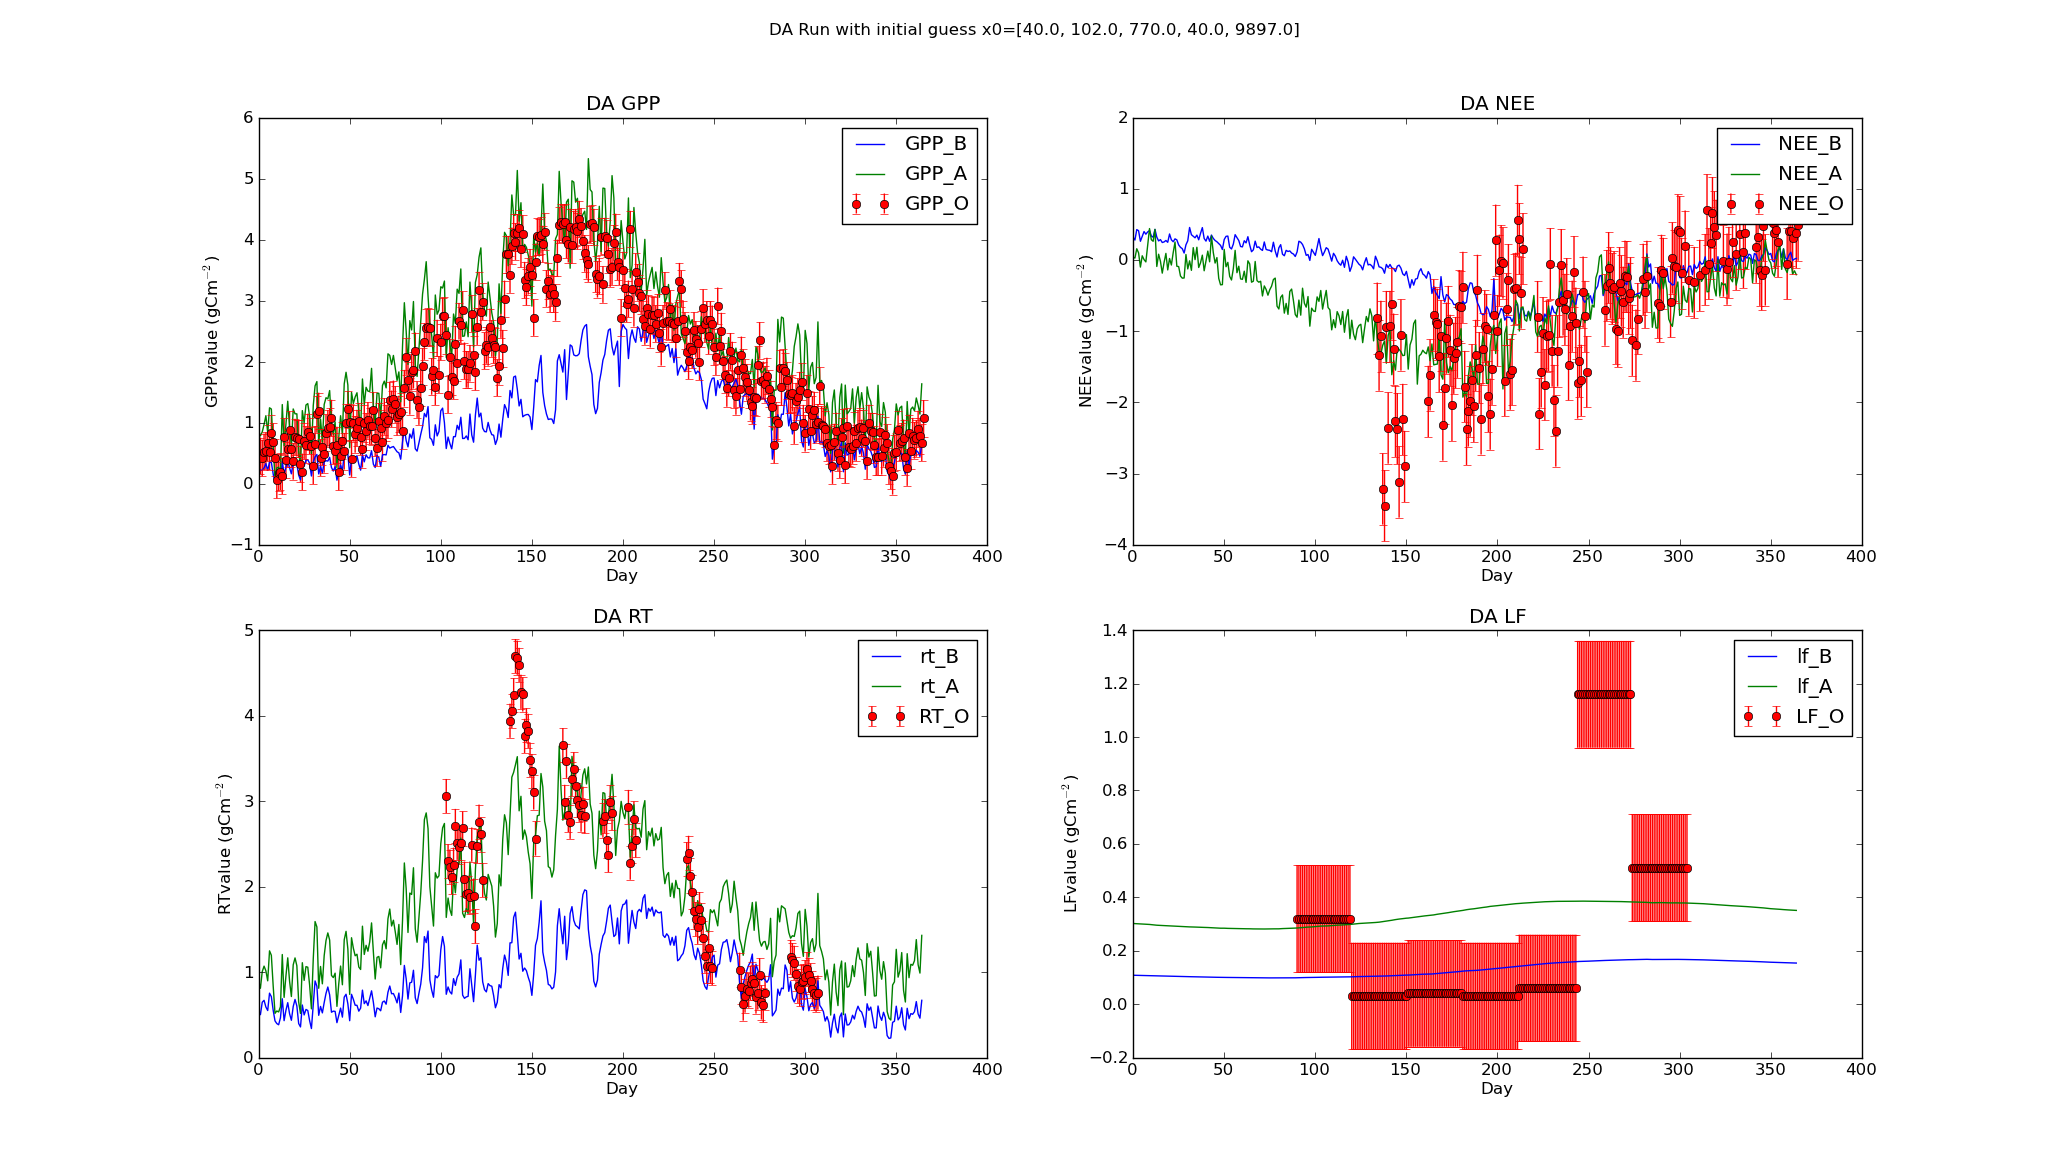
\includegraphics[width=1.04\textwidth]{DA_code_NEEonlybetterlabel.png}
    \caption{4DVAR DALEC, 365 day assimilation window, only NEE observations assimilated. }
    \label{fig:DALEC2_mod}
\end{figure}
}

%--------------SLIDE 8-----------------------------------------------------------------
\frame{
\begin{figure}[h!]
    \centering
    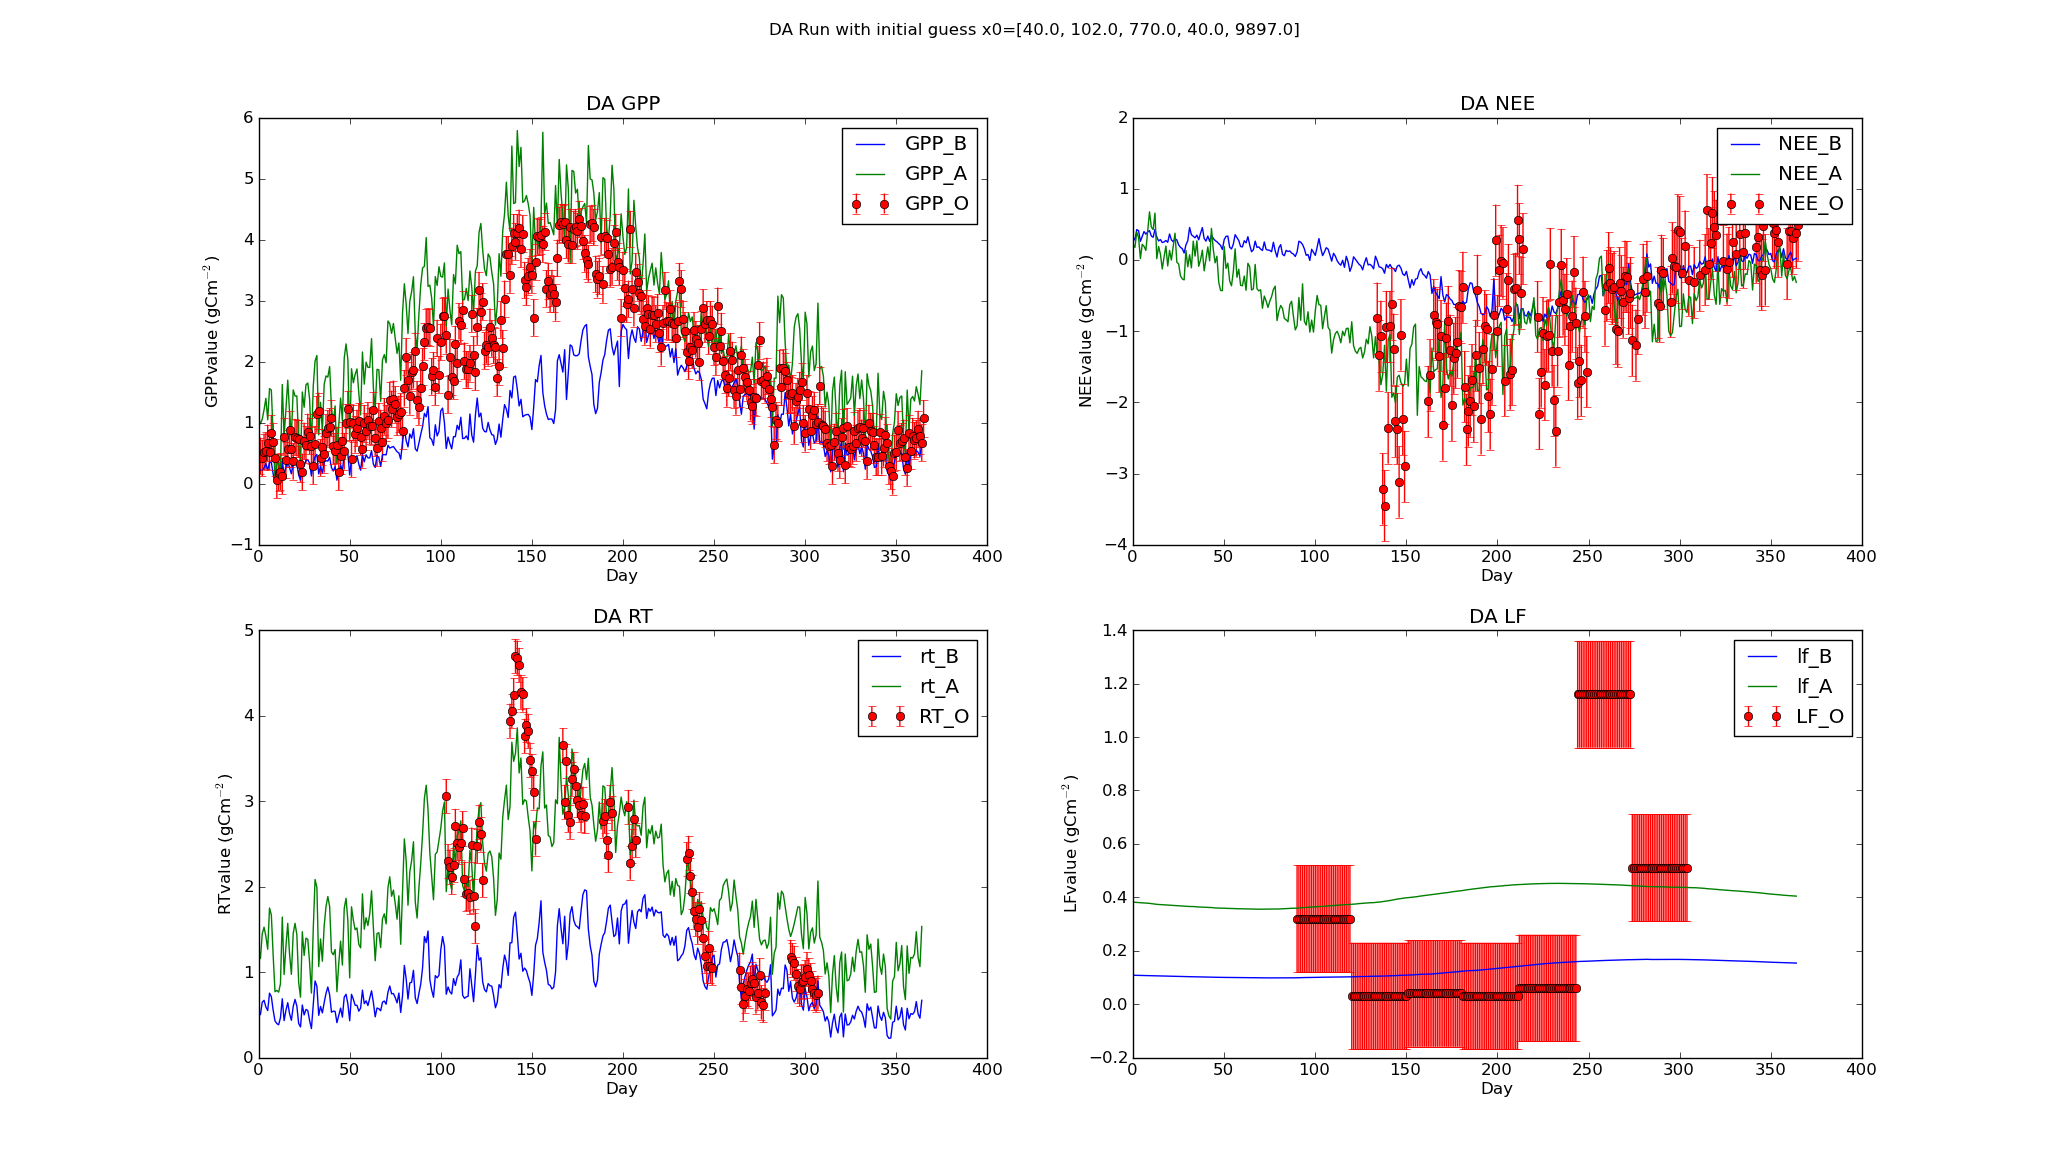
\includegraphics[width=1.04\textwidth]{DA_code_NEE&RTbetterlabel.png}
    \caption{4DVAR DALEC, 365 day assimilation window, NEE and RT observations assimilated. }
    \label{fig:DALEC2_mod}
\end{figure}
}

%--------------SLIDE 9-----------------------------------------------------------------
\frame{\frametitle{Test for DA code}
\begin{figure}[h!]
    \centering
    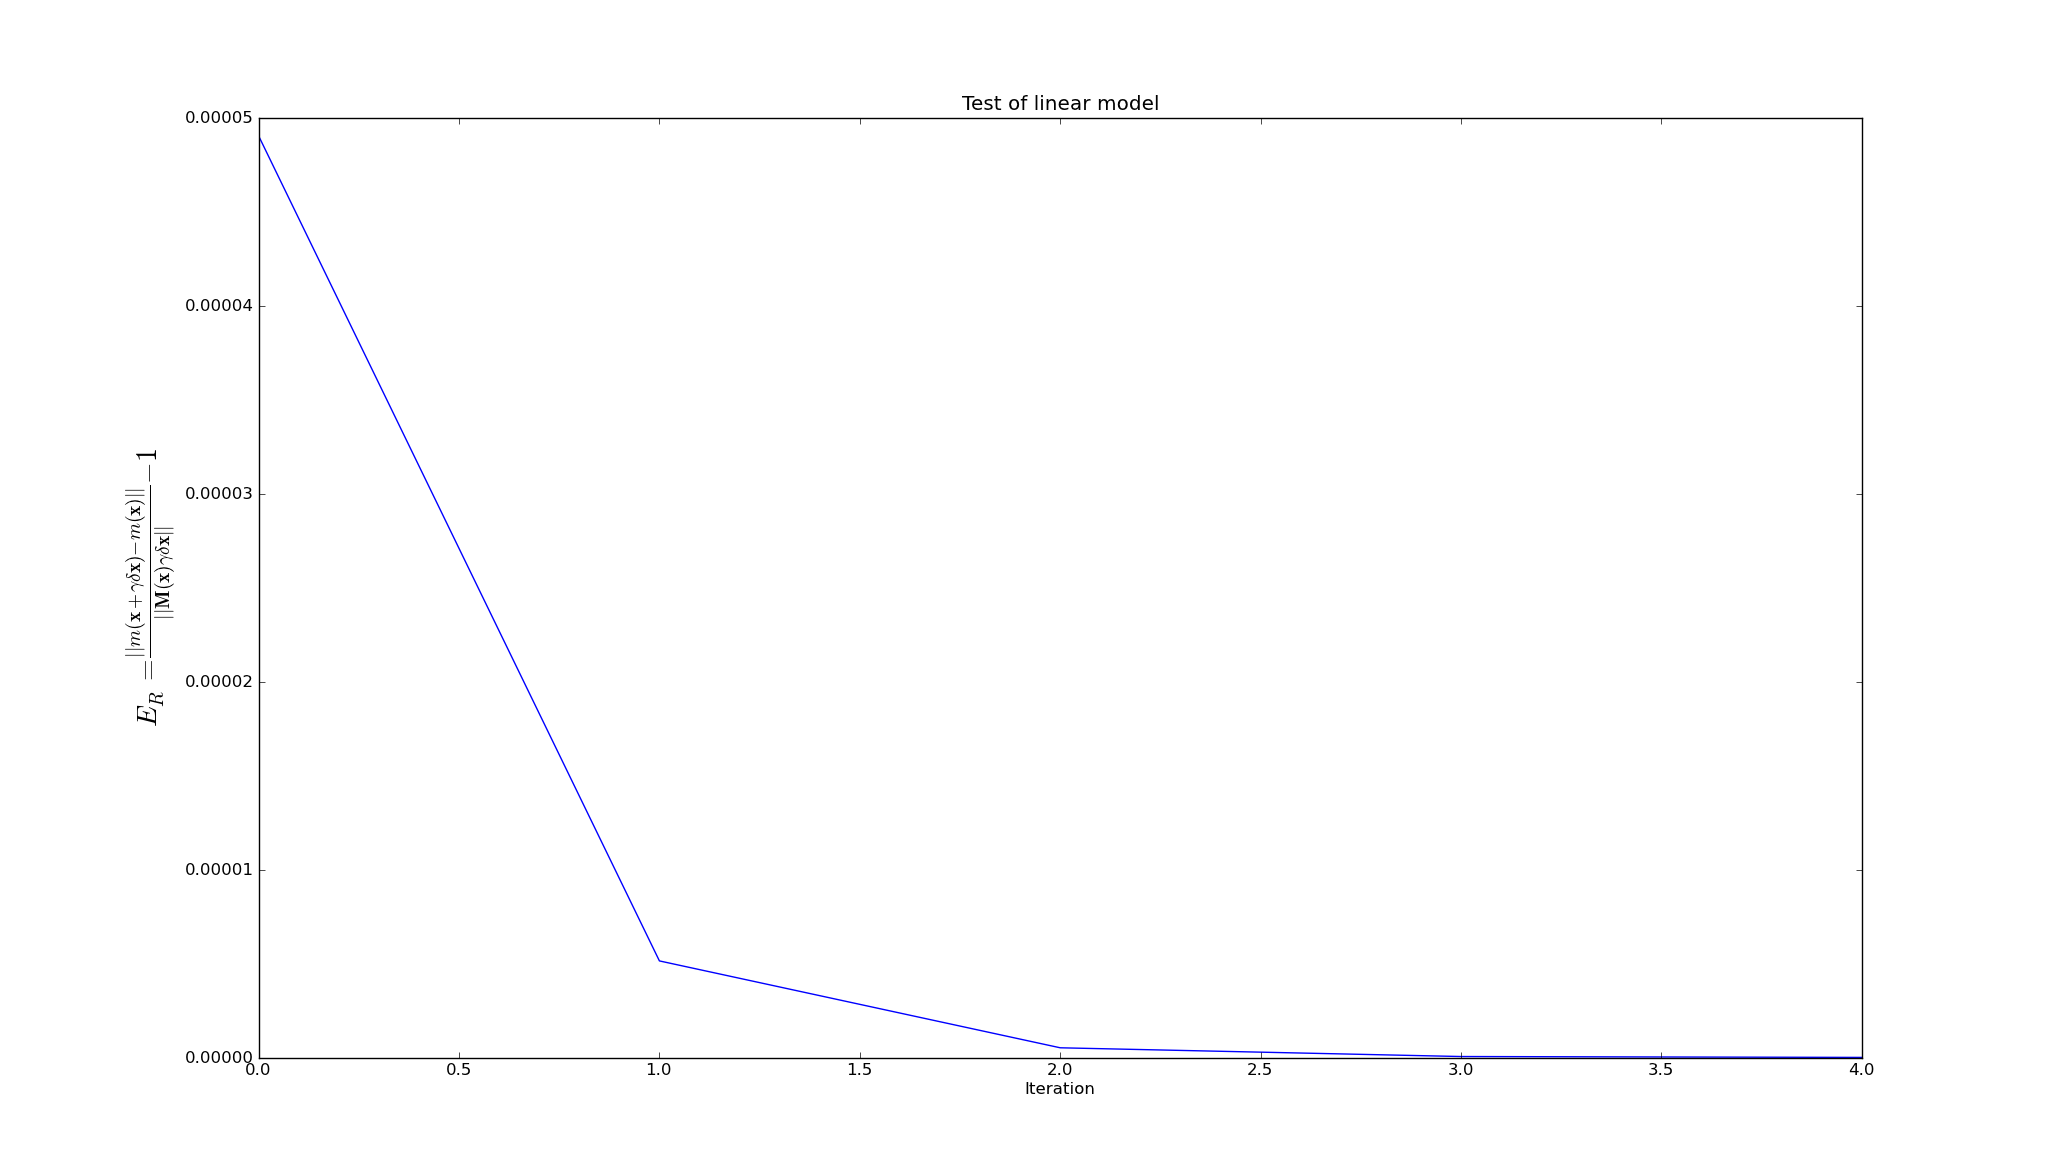
\includegraphics[width=1.\textwidth]{Test_LinMod_365norm.png}
    \caption{Linear model test for a 365 day run, $ E_R = \frac{||m({\bf x}+\gamma\delta {\bf x})-m({\bf x})||}{||{\bf M}({\bf x})\gamma\delta {\bf x}||}-1 $.}
    \label{fig:DALEC3_mod}
\end{figure}
}
\frame{
\begin{figure}[h!]
    \centering
    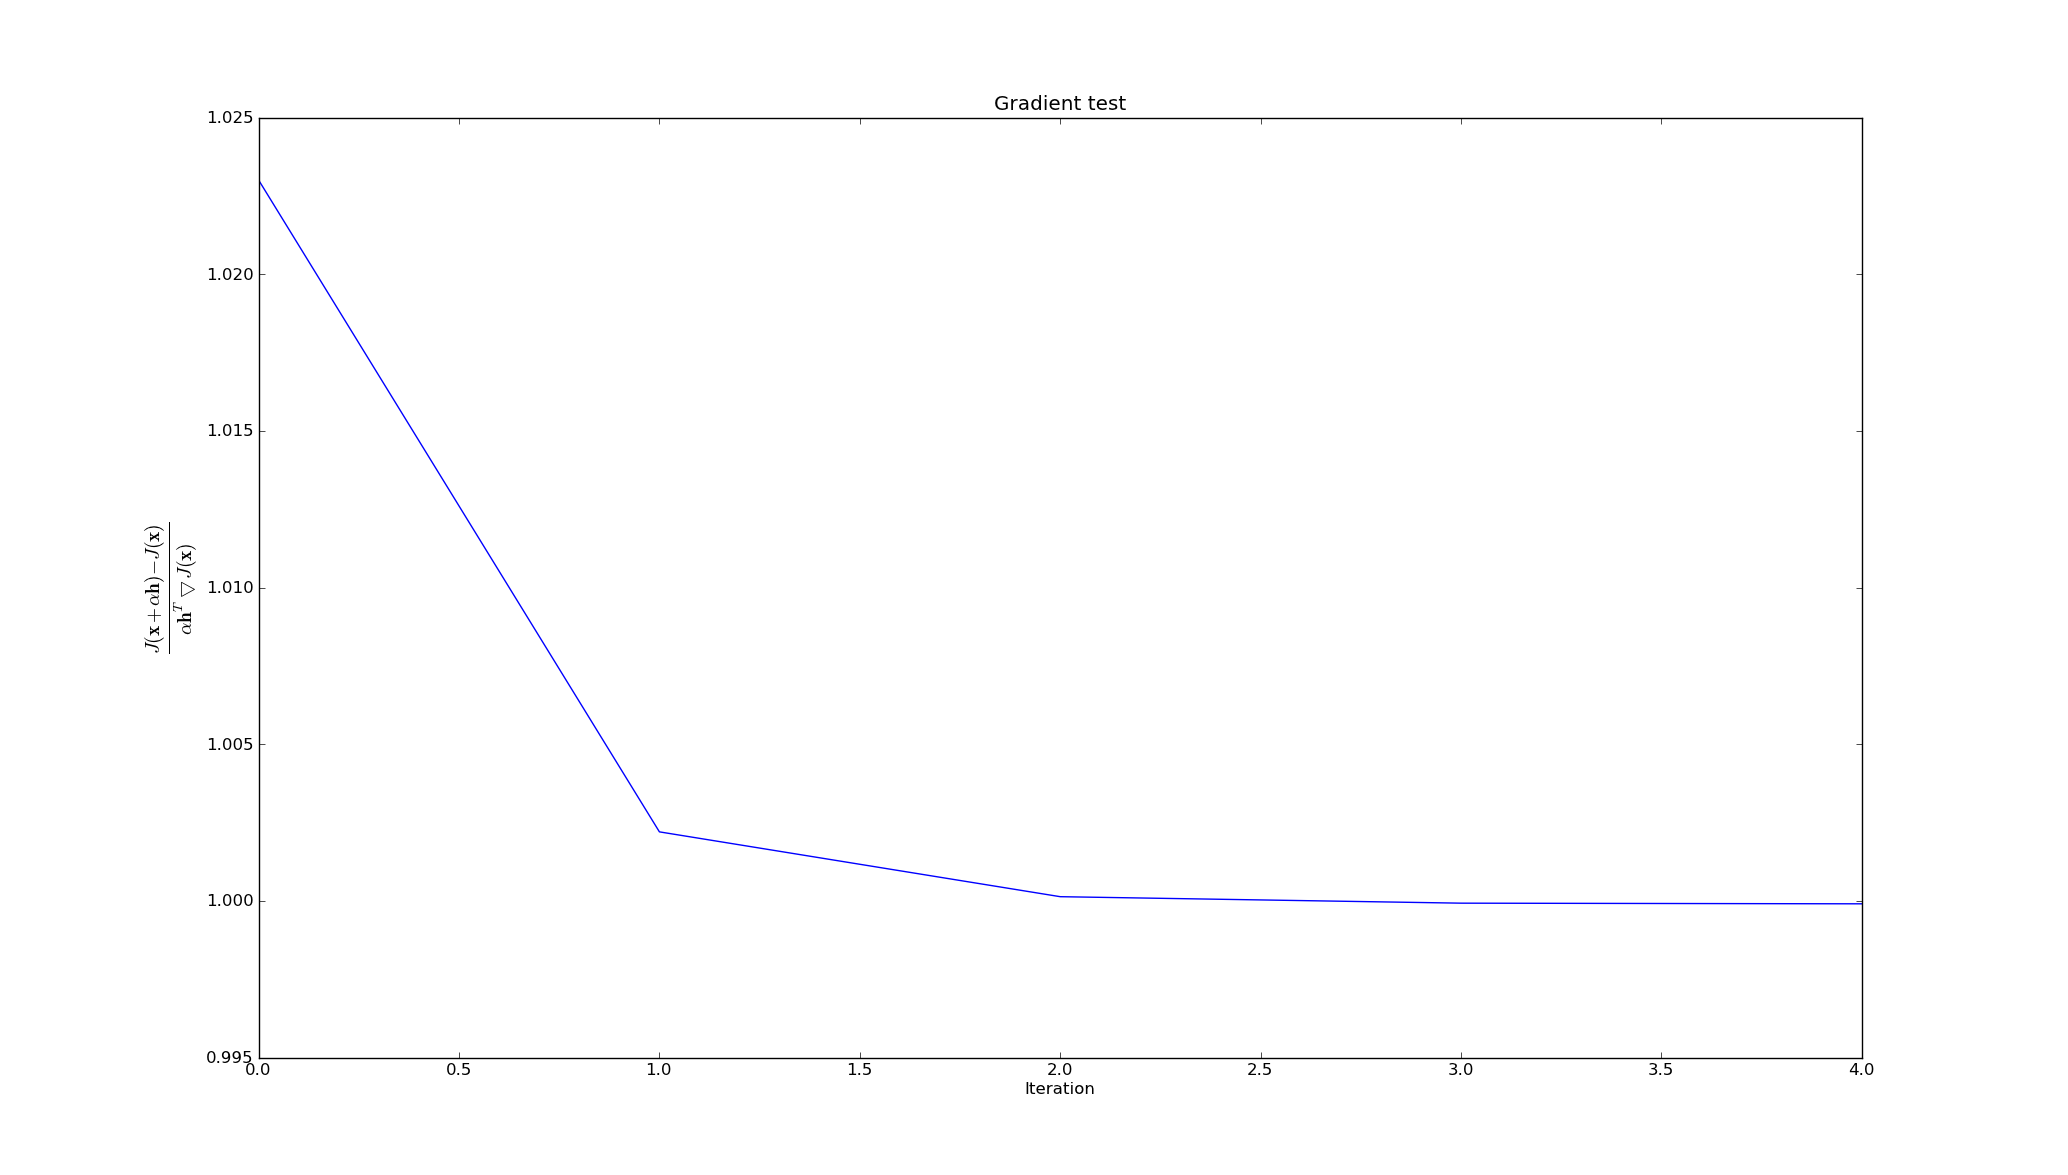
\includegraphics[width=1.\textwidth]{Gradtest_365norm.png}
    \caption{Gradient test, $\frac{J({\bf x}+\alpha{\bf h})-J({\bf x})}{\alpha{\bf h}^{T}\bigtriangledown J({\bf x})} $.}
    \label{fig:DALEC3_mod}
\end{figure}
}

\end{document}